Depending on the biological questions under investigation, to test differences between multiple conditions, \gls{tic} offers three different ways of analyzing \gls{tc} \gls{rnaseq} data and three methodologies for analyzing different biological conditions at single time point.

To do so, we took advantage of some of the mostly used and well-performing \cite{Costa-Silva2017} R/Bioconductor packages: \textit{DESeq2} \cite{Love2014}; \textit{edgeR} \cite{Robinson2009} and \textit{NOISeq} \cite{Tarazona2011, Tarazona2015}.

Exception made for \textit{NOISeq}, all the selected methods model the \gls{rnaseq} data counts for each gene as independent Negative Binomial distributions, which has been demonstrated \cite{Robinson2007} to be better suited for this data type.
At the same time, each of them differs for the statistical test implemented while approaching the biological question under investigation.
In particular, the \textit{NOISeq} method is based on a non-parametric approach, which implies that it doesn't assume any probability distribution.

In the following sections, we first present the \gls{tc} methods and then the methods for single time point gene differentiation.

\subsubsection{Time-Course DE Method 1 - \textit{LRT\_TC}}
The first method (\textit{LRT\_TC}) uses the \gls{lrt} to compare two different models in order to extract all those \glspl{deg} that invert their expression between the conditions across all the time points.

Exploiting the \gls{lrt}, as implemented in \textit{DESeq2} R/Biocnductor package, we compare two different formulas.
The first one defines the \textit{full} model where we put together the timepoints, the conditions and an interaction term between these two variables, while the second one is a reduced model where the interaction term is removed:

\[LRT \sim \frac{times+conditions+times:conditions}{times+conditions}\]

In so doing, we are able to catch all the genes with distinct expression at time 0, and inverting their expression across the conditions along the time-course experiment (figure \ref{fig:ticlrttc} provides an example of \gls{deg} detected with this method). 

\begin{figure}[H]
\centering
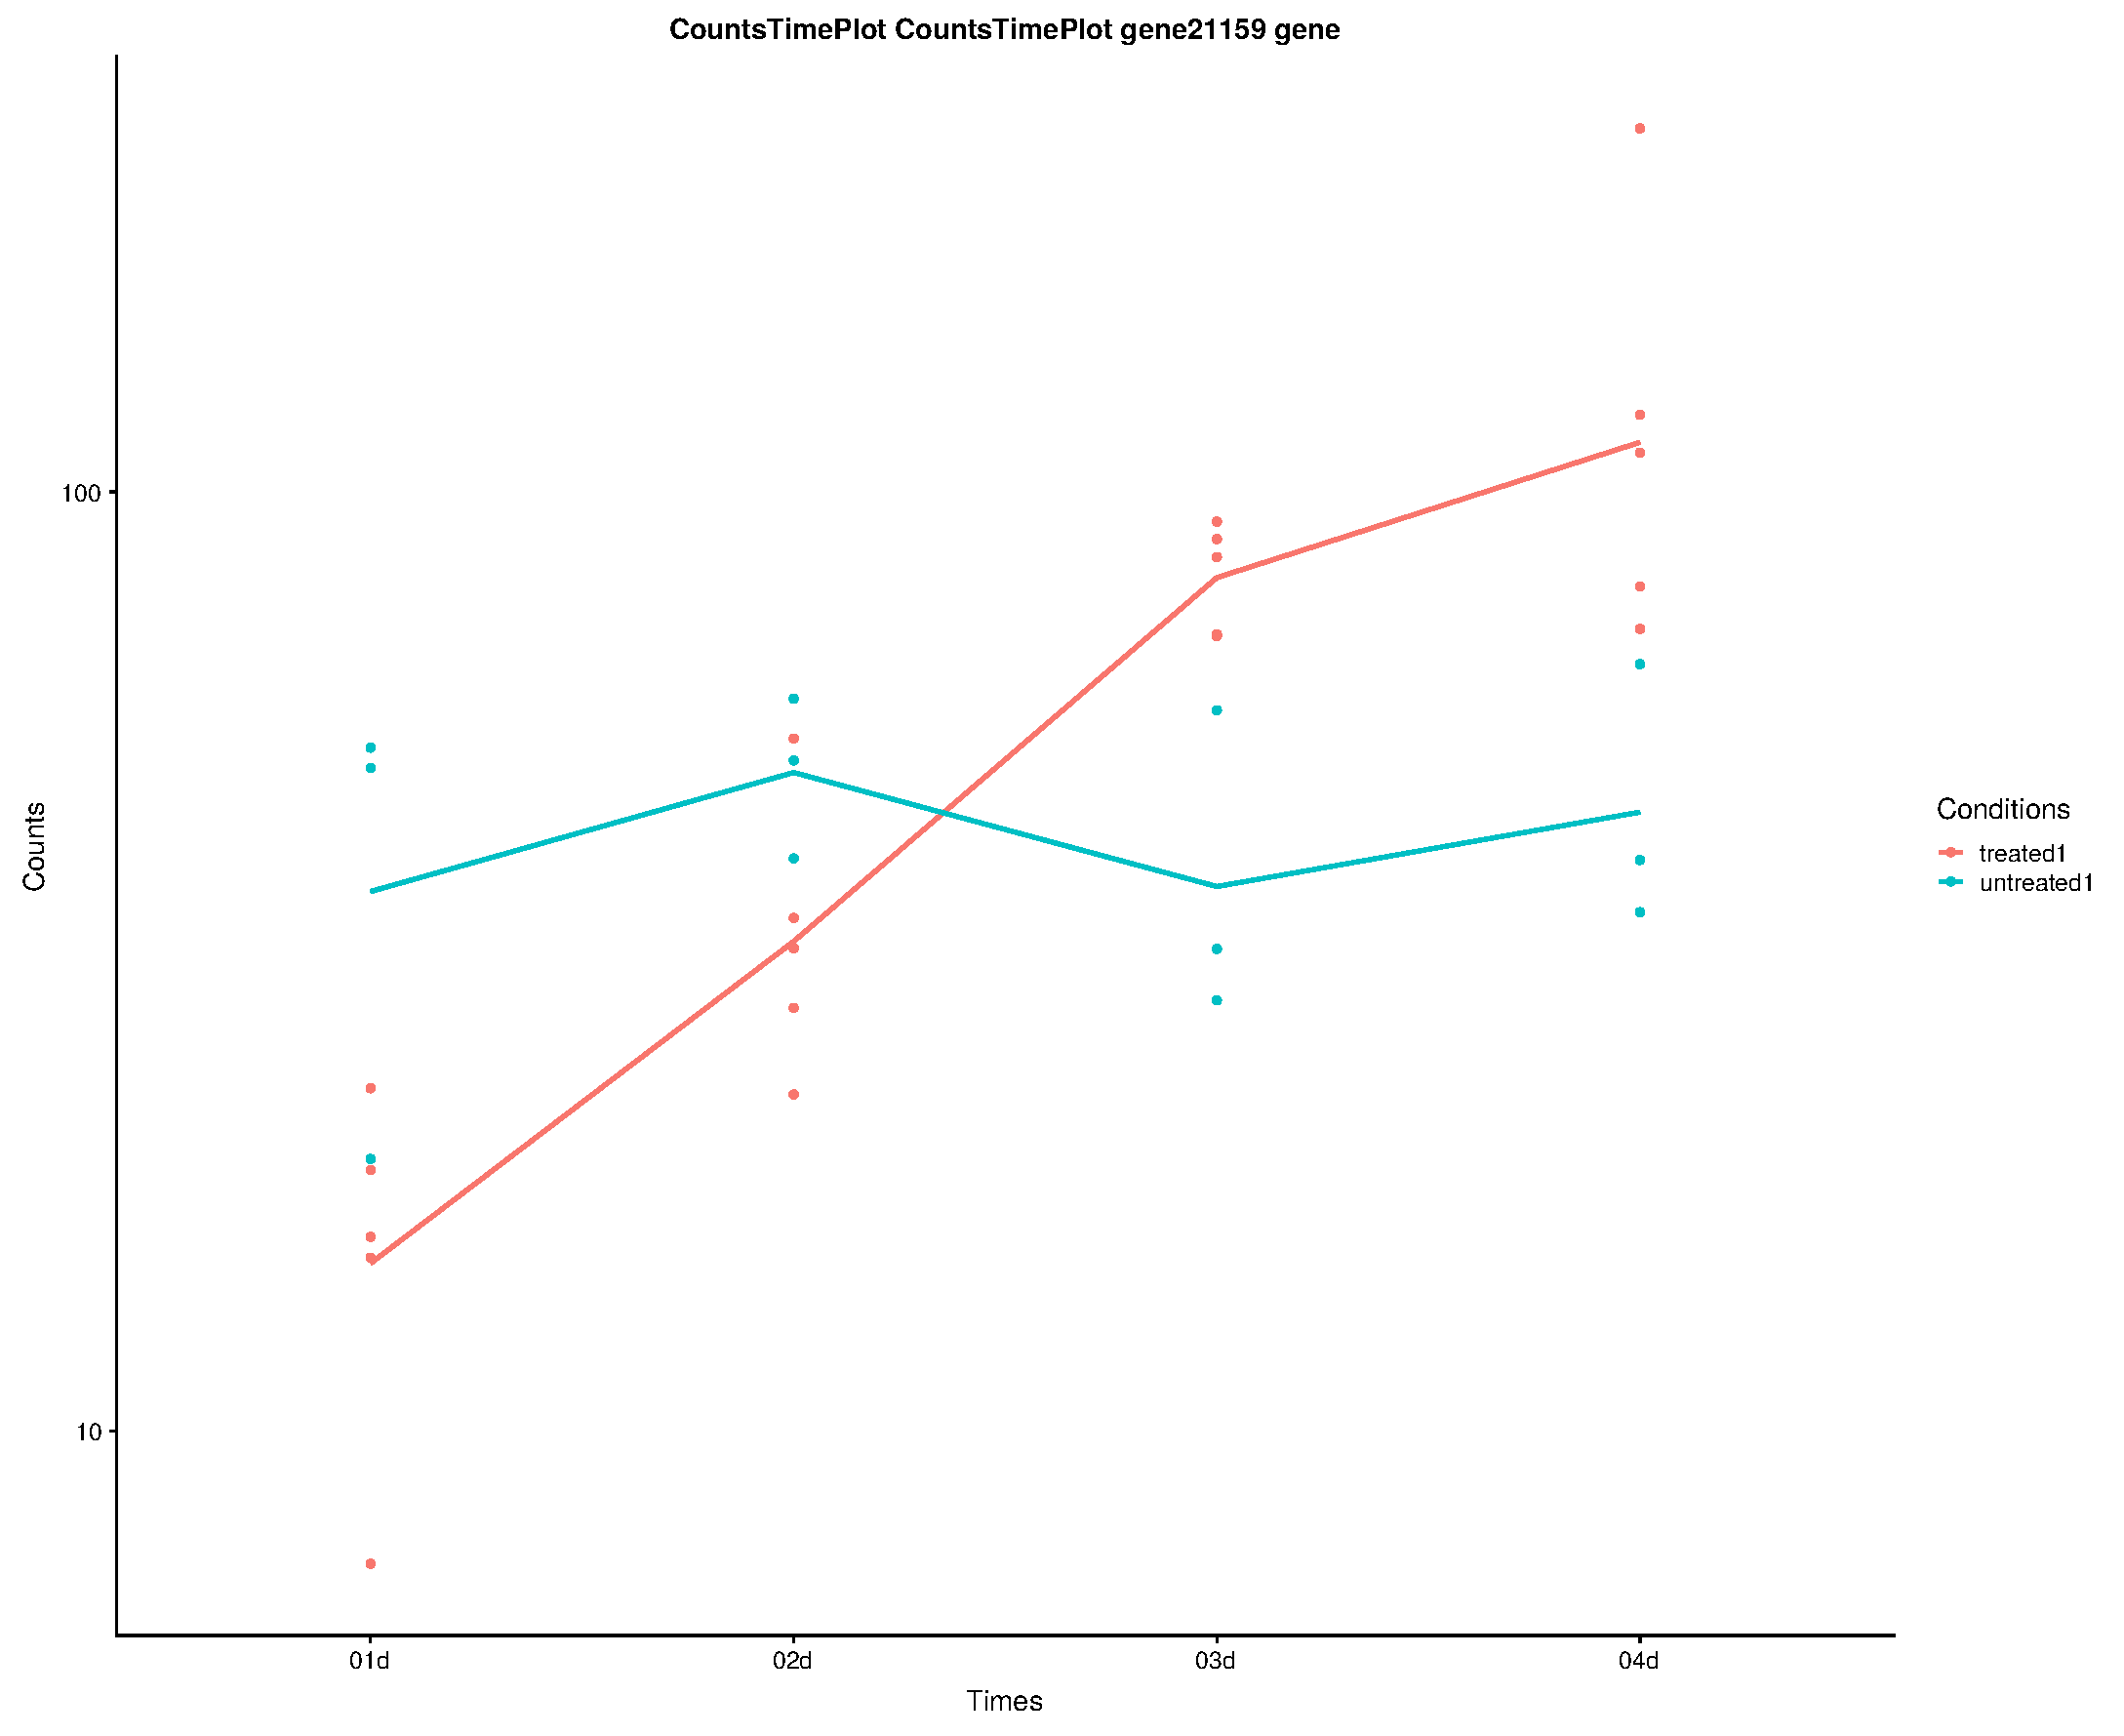
\includegraphics[width=10cm, keepaspectratio]{img/ticorser/de/trends/trend_LRT.pdf}
\caption[\gls{tic} LRT\_TC trend]{A typical trend of a \gls{deg} detected with \textit{LRT\_TC} method.
The gene trends inverts its expression between the two biological conditions across the experimental time points.}
\label{fig:ticlrttc}
\end{figure}

\subsubsection{Time-Course DE Method 2 - \textit{LRT\_T}}
The underlying idea of the second method is the same of the first one, where the difference is to remove from the \textit{reduced} formula, not only the interaction term but also the \textit{conditions} variable.

In such a way, we are able to extract all those \glspl{deg} having and preserving different expression profiles between the conditions across all the time points (figure \ref{fig:ticlrtt} provides an example of \gls{deg} detected with this method).

The first formula here defines the same \textit{full} model of the first method, while the second one is the reduced model where only the times variable appears:

\[LRT \sim \frac{times+conditions+times:conditions}{times}\]

\begin{figure}[H]
\centering
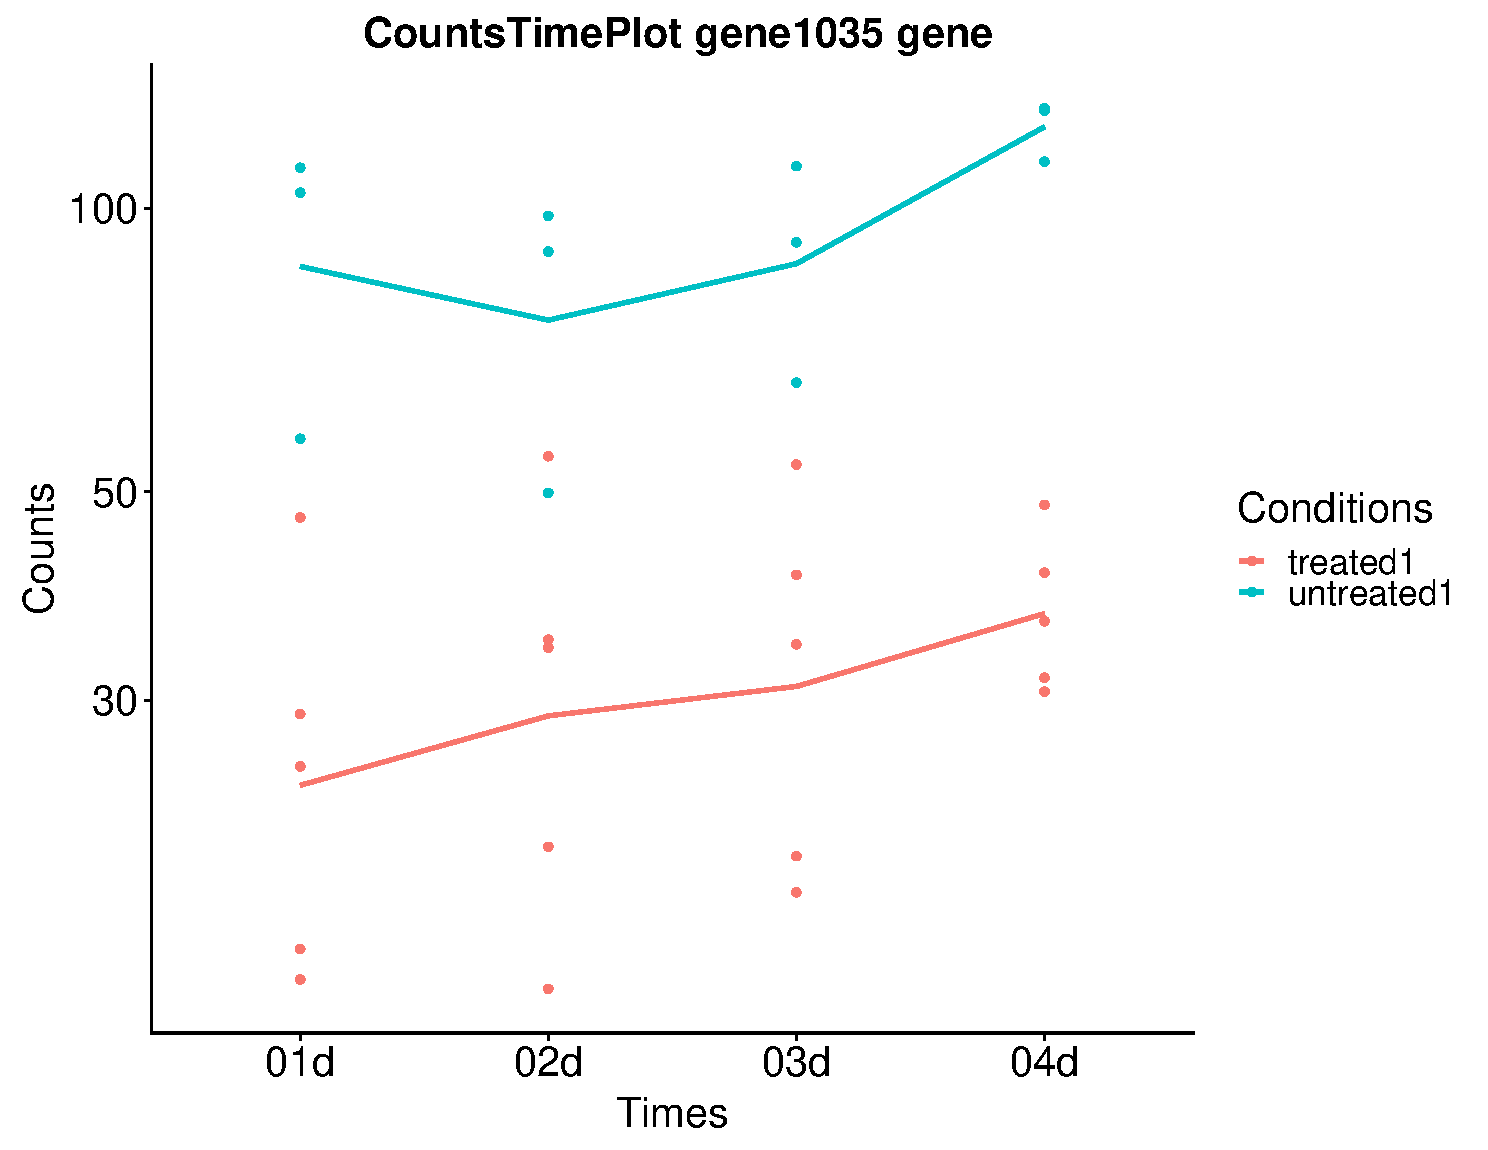
\includegraphics[width=10cm, keepaspectratio]{img/ticorser/de/trends/trend_t.pdf}
\caption[\gls{tic} LRT\_T trend]{A typical trend of a \gls{deg} detected with \textit{LRT\_T} method.
The gene has different expression between the biological conditions and maintains this expression across all the experimental time points.}
\label{fig:ticlrtt}
\end{figure}

By loosing the conditions term in the reduced formula, this method is able to catch all the \glspl{deg} detected by \textit{LRT\_TC} method, and, additionally, all the genes with different trends across all the time points.

\subsubsection{Time-Course DE Method 3 - \textit{LRT\_NOInteraction}}
Using always the \textit{DESeq2} \gls{lrt} approach, we defined a third method for the 
identification of \glspl{deg} that have different expression between the conditions across all the time points, but that maintain the same profile in both conditions (figure \ref{fig:ticlrtnotint} provides an example of \gls{deg} detected with this method).

Here the \textit{full} model defines the time points and the conditions variables without taking into account the interaction term, while the second the \textit{reduced} model presents only the time point variable:

\[LRT \sim \frac{times+conditions}{times}\]

\begin{figure}[H]
\centering
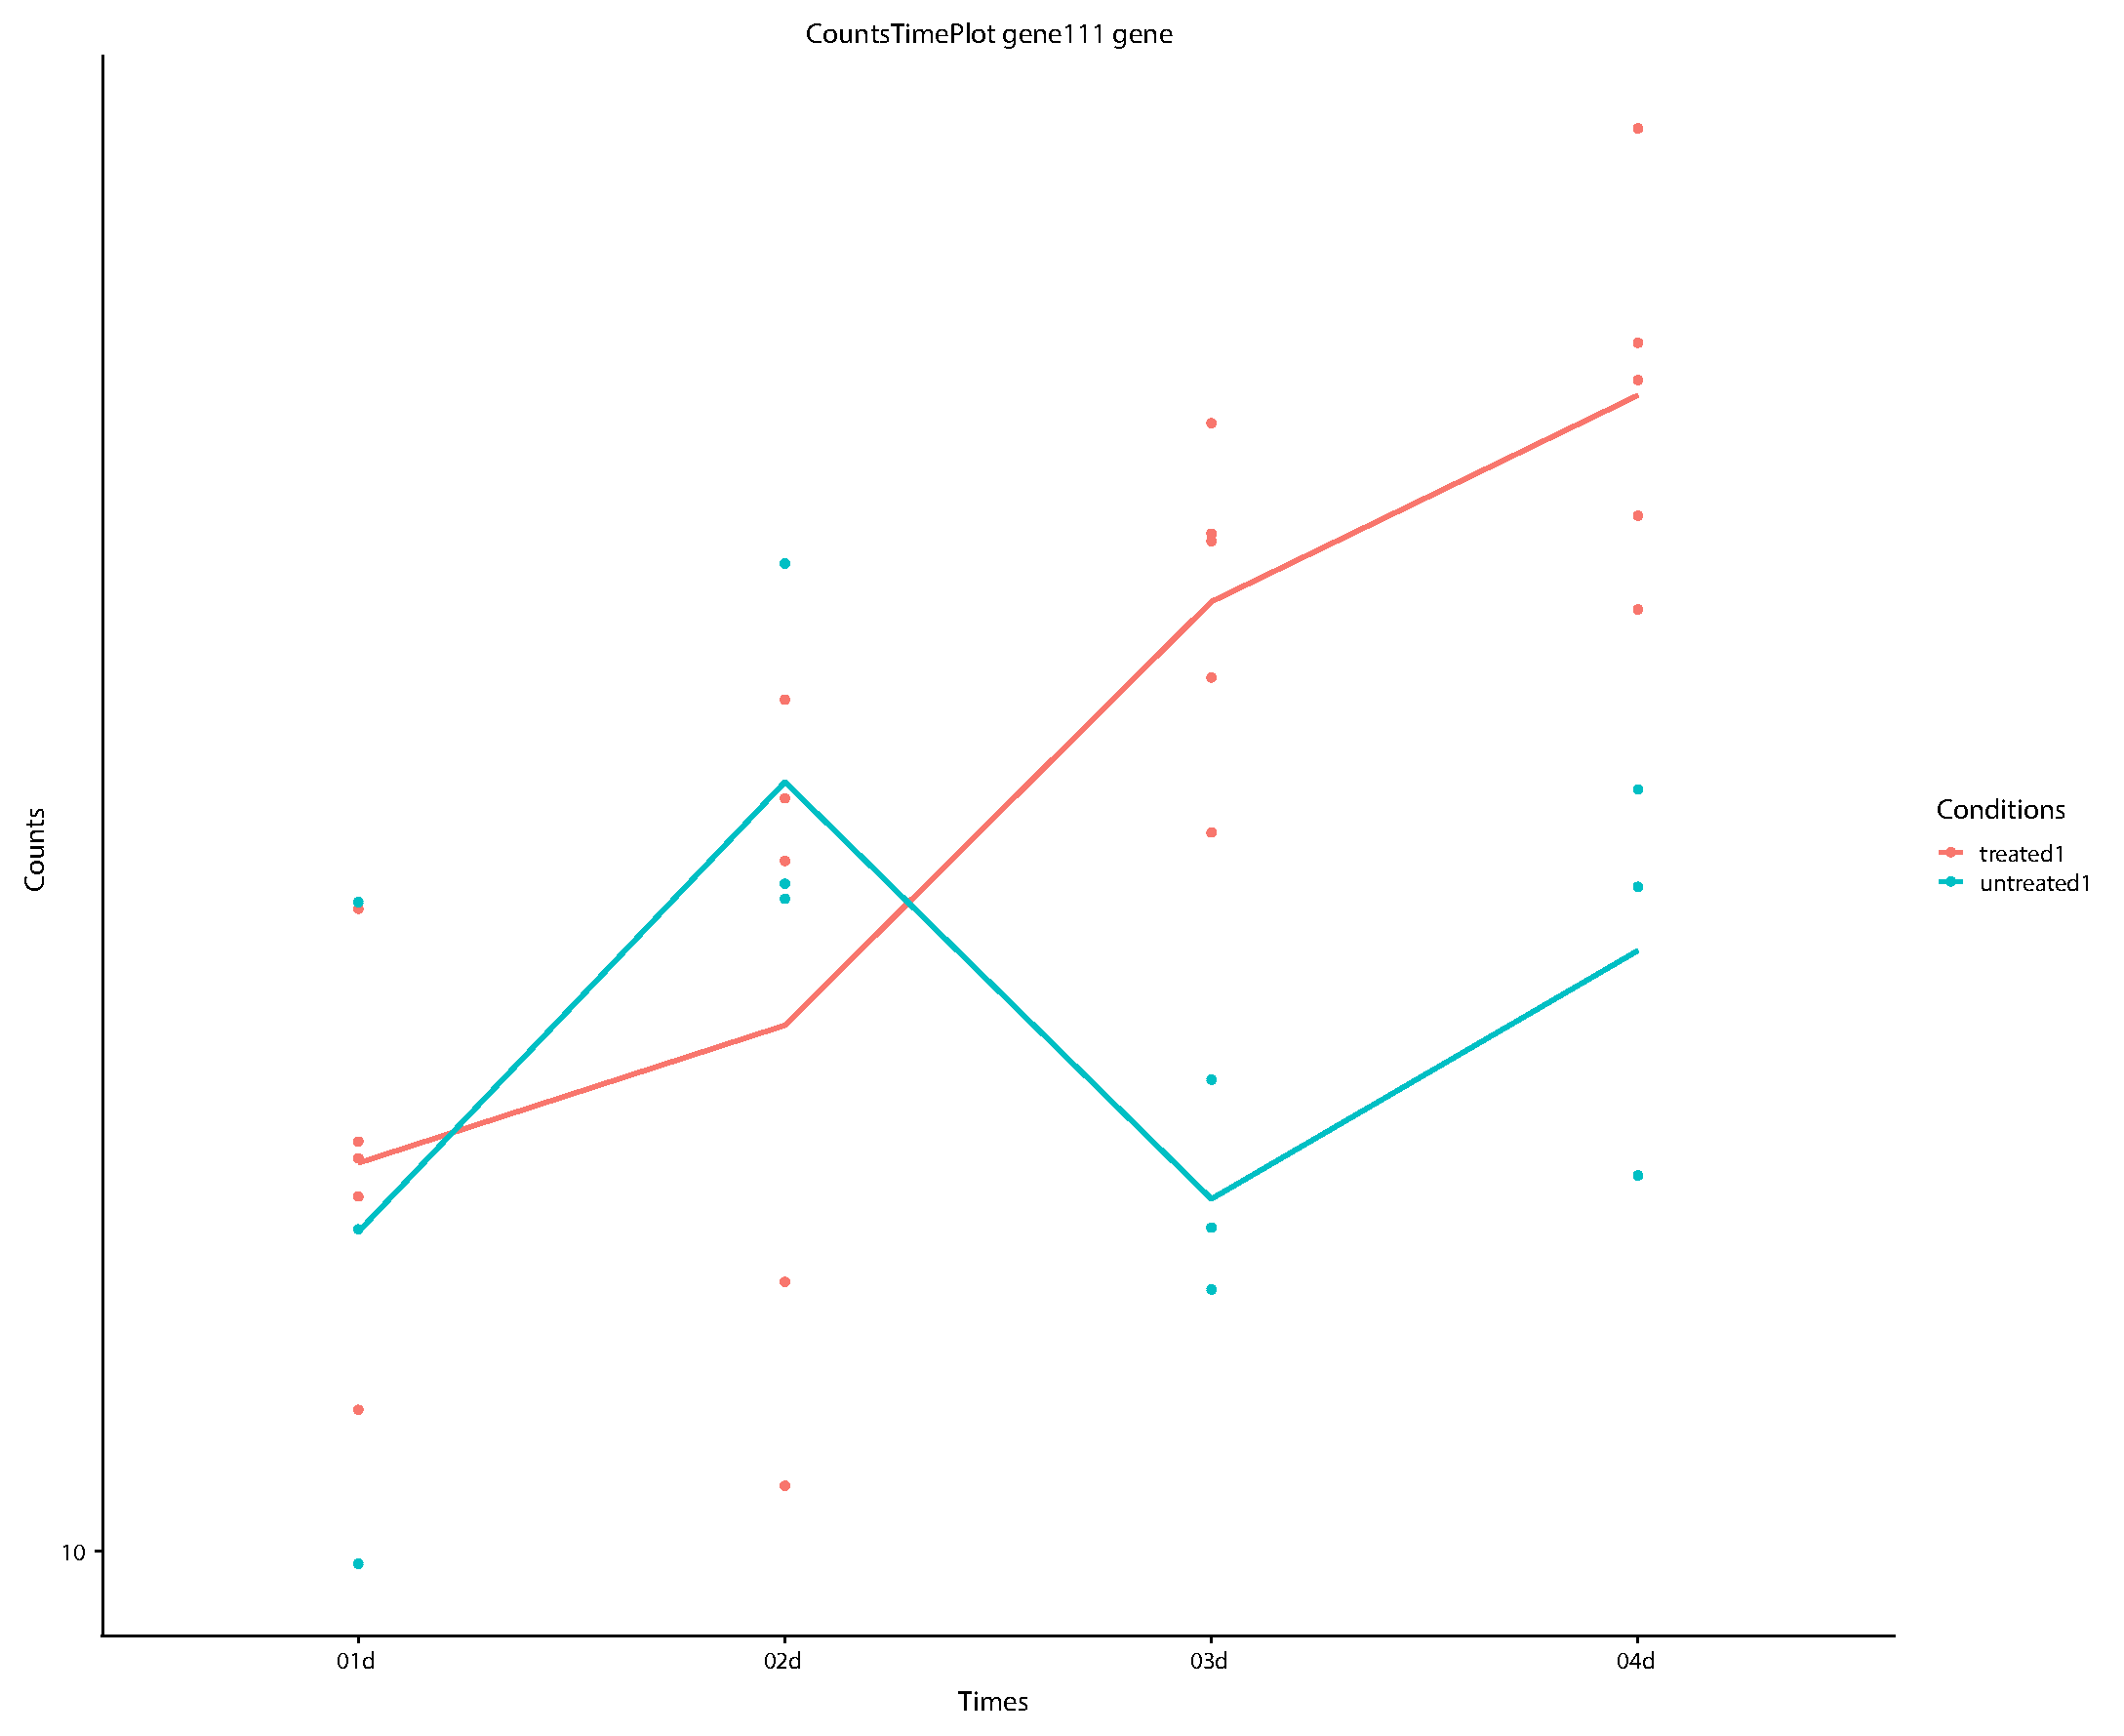
\includegraphics[width=10cm, keepaspectratio]{img/ticorser/de/trends/trend_noint.pdf}
\caption[\gls{tic} LRT\_NOInteraction trend]{A typical trend of a \gls{deg} detected with \textit{LRT\_NoInteraction} method.}
\label{fig:ticlrtnoint}
\end{figure}

Because of the absense of the interaction term, this method detects the highest number of \glspl{deg} expressing difference between the conditions, but not taking into account this difference across the time points.
Indeed, it seems to be able to detect several genes in common with other \gls{lrt} methods, showing an high number of \glspl{deg} detected by itself.

\subsubsection{Time-Course DE Method - \textit{Wald}}

After using the \gls{lrt} test, the \textit{DESeq2} package, thanks to its results data structure, offers the possibility to apply the \textit{Wald} test on the previously computed \gls{lrt} results, by specifying the contrasts to be tested.

In such a way it is possible to test the differences between the biological conditions at a single time point.

In particular, we designed \gls{tic} to automatically apply this additional test and return the \glspl{deg} expressing differences between the biological conditions at time 0.

From some preliminary tests, this method seems to be able to detect mostly the same \glspl{deg} detected with the \textit{LRT\_NOInteraction} method.

%\subsubsection{Time-Course DE Method 4 - \textit{nextMASigPro}}
%
%The fourth method takes advantage of the \gls{glm} with Negative Binomial distribution as defined in the \textit{maSigPro} R/Bioconductor package.
%This method, unlike the previous ones, allows detecting all the \glspl{deg} showing any kind of differences between the conditions across all the time points.
%Indeed, as suggested by the \textit{maSigPro} authors is a good norm to cluster the genes to better understand which is their singular behaviour.


\subsubsection{Single DE Methods}

To account for fixed time point experiment, we implemented functionalities for helping also the exploration of this aspect, using three different methodologies.
 
%Our package offers a way to analyze the differences between the conditions at  single time point, offering three different methodologies.

By using the \lstinline!differentiateConditions! function, it is possible to choose between the \textit{edgeR}, \textit{DESeq2}, \textit{NOISeq} and \textit{NOISeqBio}.

In case of \textit{edgeR} we decided to use the \textit{Quasi-Likelihood} method for the differential expression.
While, for this specific case, when using \textit{DESeq2}, we choose the \textit{Wald} test, as suggested by the authors.

The \textit{NOISeq} package offers the possibility to discriminate between \textit{biological} and \textit{technical} replicates, computing a posterior probability in both cases, but applying different hypothesis tests.

In case of \textit{technical} replicates, the \textit{NOISeq} method has to be applied, considering that it requires the full count matrix, within low expressed genes, in order to be able to properly estimate the data distribution.
While when biological replicates are available it is more indicated to apply \textit{NOISeqBio}, which requires at least 3 replicates per condition.



